%\documentclass[a4paper,superscriptaddress,11pt]{quantumarticle}
\documentclass[aps,twocolumn,longbibliography,english,superscriptaddress,prr]{revtex4-1}
%\documentclass[a4paper,superscriptaddress,11pt]{article}
\pdfoutput=1
\usepackage[colorlinks=true,urlcolor=blue,citecolor=blue,linkcolor=blue]{hyperref}
\usepackage[english]{babel}
\usepackage[utf8]{inputenc}
\usepackage[T1]{fontenc}
\usepackage{amssymb}
\usepackage{tabularx}
\usepackage{upquote}
%\usepackage{multicol}
%\usepackage{caption}
\usepackage[plain]{algorithm}
\usepackage{algpseudocode}
\usepackage{rotating}
%\usepackage{cite}
\usepackage{booktabs}
%\usepackage{unicode-math}
%\usepackage{algorithm}% http://ctan.org/pkg/algorithm
%\usepackage{algpseudocode}% http://ctan.org/pkg/algpseudocode
\usepackage{xcolor}% http://ctan.org/pkg/xcolor
\makeatletter
\newsavebox{\@brx}
\newcommand{\llangle}[1][]{\savebox{\@brx}{\(\m@th{#1\langle}\)}%
  \mathopen{\copy\@brx\kern-0.5\wd\@brx\usebox{\@brx}}}
\newcommand{\rrangle}[1][]{\savebox{\@brx}{\(\m@th{#1\rangle}\)}%
  \mathclose{\copy\@brx\kern-0.5\wd\@brx\usebox{\@brx}}}
\makeatother

\usepackage{bbm}
\usepackage{jlcode}
\usepackage{graphicx, subfigure}
\usepackage{amsmath,color,amsthm}
\usepackage{mathrsfs}
\usepackage{float}
\usepackage[normalem]{ulem}
\usepackage{indentfirst}
\usepackage{txfonts}
\usepackage{listings}
\lstset{
    language=Julia,
    basicstyle=\ttfamily\footnotesize,
    numberstyle=\scriptsize,
    % numbers=left,
    backgroundcolor=\color{gray!10},
    frame=single,
    tabsize=2,
    rulecolor=\color{black!30},
    title=\lstname,
    escapeinside={\%(*}{*)},
    breaklines=true,
    breakatwhitespace=true,
    framextopmargin=2pt,
    framexbottommargin=2pt,
    extendedchars=true,
    inputencoding=utf8,
    columns=fullflexible,
}

\usepackage[epsilon, tsrm, altpo]{backnaur}

\tolerance=1
\emergencystretch=\maxdimen
\hyphenpenalty=1000
\hbadness=1000

\makeatletter

%%%%%%%%%%%%%%%%%%%%%%%%%%%%%% User specified LaTeX commands.

%Journal reference.  Comma sets off: name, vol, page, year
\def\journal #1, #2, #3, 1#4#5#6{{\sl #1~}{\bf #2}, #3 (1#4#5#6) }
\def\pr{\journal Phys. Rev., }
\def\prb{\journal Phys. Rev. B, }
\def\prl{\journal Phys. Rev. Lett., }
\def\pl{\journal Phys. Lett., }
%\def\np{\journal Nucl. Phys., }


%%%%%%%%%%%%%%%%%%%%%%%%%%%%%%%%%%%%%%%%%%%%%%%%%%%%%%%%%%%%%%%%%%%%%%%%%%%%%%%%%%%%%%%%%%%%%%%%%%%%%%%%%%%%%%%%%%%%%%%%%%%%%%%%%%%%%%%%%%%%%%%%%%%%%%%%%%%%%%%%%%%%%%%%%%%%%%%%%%%%%%%%%%%%%%%%%%%%%%%%%%%%%%%%%%%%%%%%%%%%%%%%%%%%%%%%%%%%%%%%%%%%%%%%%%%%


%\usepackage{CJK}
%\usepackage[colorlinks, citecolor=blue]{hyperref}
\DeclareMathOperator*{\argmax}{arg\,max}

%%%%%% Shortcut related
\newcommand{\<}{\langle}
\renewcommand{\>}{\rangle}
\newcommand{\out}{{O}}
\newcommand{\inp}{{I}}
\newcommand{\pluseq}{\mathrel{+}=}
\newcommand{\minuseq}{\mathrel{-}=}
\newcommand{\vx}{{\vec x}}
\newcommand{\vy}{{\vec y}}
%%%%%% Convention related
\newcommand{\SWAP}{{\rm SWAP}}
\newcommand{\CNOT}{{\rm CNOT}}
\newcommand{\X}{{\rm X}}
\renewcommand{\H}{{\rm H}}
\newcommand{\Rx}{{\rm Rx}}
\renewcommand{\v}[1]{{\bf #1}}
\newcommand{\dataset}{{\mathcal{D}}}
\newcommand{\wfunc}{{\psi}}
\newcommand{\SU}{{\rm SU}}
\newcommand{\UU}{{\rm U}}
\newcommand{\thetav}{{\boldsymbol{\theta}}}
\newcommand{\gammav}{{\boldsymbol{\gamma}}}
\newcommand{\thetai}{{\theta^\alpha_l}}
\newcommand{\Expect}{{\mathbb{E}}}
\newcommand{\Tr}{{\rm Tr}}
\newcommand{\etc}{{\it etc~}}
\newcommand{\etal}{{\it etal~}}
\newcommand{\xset}{\mathbf{X}}
\newcommand{\fl}{\texttt{fl}}
\newcommand{\pdata}{\mathbf{\pi}}
\newcommand{\q}{\mathbf{q}}
\newcommand{\epdata}{\mathbf{\hat{\pi}}}
\newcommand{\gammaset}{\boldsymbol{\Gamma}}
\newcommand{\ei}{{\mathbf{e}_l^\alpha}}
\newcommand{\vtheta}{{\boldsymbol{\theta}}}
\newcommand{\sigmag}{{\nu}}
\newcommand{\sigmai}[2]{{\sigma^{#2}_{#1}}}
\newcommand{\qi}[1]{{q^{\alpha_{#1}}_{#1}}}
\newcommand{\BAS}{Bars-and-Stripes}
\newcommand{\circled}[1]{\raisebox{.5pt}{\textcircled{\raisebox{-.9pt} {#1}}}}

\newcommand{\qexpect}[1]{{\left\langle #1\right\rangle}}
\newcommand{\expect}[2]{{\mathop{\mathbb{E}}\limits_{\substack{#2}}\left[#1\right]}}
\newcommand{\var}[2]{{\mathop{\mathrm{Var}}\limits_{\substack{#2}}\left(#1\right)}}
\newcommand{\pshift}[1]{{p_{\thetav+#1}}}
\newcommand{\upcite}[1]{\textsuperscript{\cite{#1}}}
\newcommand{\Eq}[1]{Eq.~(\ref{#1})}
\newcommand{\Fig}[1]{Fig.~\ref{#1}}
\newcommand{\Tbl}[1]{Table~\ref{#1}}
\newcommand{\Sec}[1]{Sec.~\ref{#1}}
\newcommand{\App}[1]{Appendix \ref{#1}}
\newcommand{\bra}[1]{\mbox{$\left\langle #1 \right|$}}
\newcommand{\ket}[1]{\mbox{$\left| #1 \right\rangle$}}
\newcommand{\braket}[2]{\mbox{$\left\langle #1 | #2 \right\rangle$}}
\newcommand{\tr}[1]{\mathrm{tr}\mbox{$\left[ #1\right]$}}

\newcommand{\ra}[1]{\renewcommand{\arraystretch}{#1}}

%%%%%% Comment related
\newcommand{\red}[1]{[{\bf  \color{red}{LW: #1}}]}
\newcommand{\xred}[1]{[{\bf  \color{red}{\sout{LW: #1}}}]}
\newcommand{\blue}[1]{[{\bf  \color{blue}{JG: #1}}]}
\newcommand{\xblue}[1]{[{\bf  \color{blue}{\sout{JG: #1}}}]}
\newcommand{\material}[1]{\iffalse[{\bf  \color{cyan}{Material: #1}}]\fi}

\newtheorem{theorem}{\textit{Theorem}}
\theoremstyle{definition}\newtheorem{definition}{\textit{Definition}}

\makeatother

\begin{document}
\title{Instruction level automatic differentiation on a reversible Turing machine}

%\author{Jin-Guo Liu\thanks{cacate0129@iphy.ac.cn}\\
%Institute of Physics, Chinese Academy of Sciences,\\Beijing 100190, China\\
%\And
%Hong-Xuan Zhao-Wang\\
%Department of Computer Science, University of Tsukuba
%}
%\author{Lei Wang}
%\email{wanglei@iphy.ac.cn}
%\affiliation{Institute of Physics, Chinese Academy of Sciences, Beijing 100190, China}
%\affiliation{CAS Center for Excellence in Topological Quantum Computation, University of Chinese Academy of Sciences, Beijing 100190, China}
%\affiliation{Songshan Lake Materials Laboratory, Dongguan, Guangdong 523808, China}

\author{Jin-Guo Liu}
\email{cacate0129@iphy.ac.cn}
\affiliation{Institute of Physics, Chinese Academy of Sciences, Beijing 100190, China}

\author{Taine Zhao}
\affiliation{Department of Computer Science, University of Tsukuba}

\begin{abstract}
    This paper considers instruction level differential programming, i.e. knowing only the backward rule of basic instructions like +, -, * and /, differentiate a program with proper performance. We will review briefly why instruction level automatic differentiation is hard for current machine learning package even for a source to source automatic differentiation package. Then we propose a reversible Turing machine implementation to achieve instruction level automatic differentiation.
\end{abstract}


\maketitle

%\begin{multicols}{2}
\section{Automatic differentiation}
    There are two modes of automatic differentiation (AD)~\cite{Hascoet2013}, the tangent mode and the adjoint mode.
    Consider a multi-in multi-out function $\vy = f(\vx)$, the tangent mode computes a column of its Jacobian $\frac{\partial \vy}{\partial x_i}$ efficiently, where $x_i$ is one of the input variables.
Whereas the adjoint mode computes a row of Jacobian $\frac{\partial y_i}{\partial \vec{x}}$ efficiently.

Most popular automatic differentiation package implements the adjoint mode differentation, since the adjoint mode is computational more efficient in variational applications, where the output loss is always a scalar.
However, implementing adjoint mode AD requires a program's intermediate state backward, which requires cahing extra informations during computation
\begin{enumerate}
    \item computational graph,
    \item and intermediate result caching.
\end{enumerate}
The computational graph is a DAG that stores function calls from inputs to results. Intermediate results are usually the input variable of a function, it is nessesary to compute the adjoint of the function.
In Pytorch~\cite{Paszke2017} and Flux~\cite{Innes2018}, every variable (tensor) has a tracker field that stores its parent (input data and function that generate this variable) information in computational graph and intermediate state. TensorFlow~\cite{Tensorflow2015} implements a static computational graph before actual computing happens.
Source to source automatic differentiation package Zygote~\cite{Innes2019} use a intermediate representation SSA as the computational graph, so that it can back propagate over a native julia code. Its intermediate caching is handled by a global storage.

Some problems are observed in most machine learning packages. First of all, these package requires a lot definitions of primitives.
    These primitive functions are compiled to instructions, these instructions are from a finite set of `+', `-', `*', `/', conditional jump statements et. al. With instruction level computational graph, it is possible to obtain gradients like \texttt{exp}, or even linear algebras functions like singular value decomposition and eigenvalue decomposition~\cite{Seeger2017,Wan2019,Hubig2019} automatically. The recent development of backward rules of linear algebra functions greatly change the field of physics~\cite{Xie2020,Liao2019}. However, these rules are generated manually.
    Secondly, inplace functions are not handled properly in the language of computational graph, even in source to source AD engine Zygote, it is not trivil. This costs unnessesary allocations and make the memory wall problem even more sevire.~\cite{memorywall}
    Thridly, obtaining higher order gradients are not efficient in these packages. In Pytorch and Tensorflow, people back propagate the whole program to obtain lower order gradients, which has exponential overhead with respect to the order of gradients. A better approach to obtain higher order gradients is through Taylor propagation ~\cite{Bettencourt2019}. However Taylor propagation requires writing rules for all primitives. Besides the exponential overhead, the sorce to source AD engine Zygote suffers from the significant overhead of just in time compiling.

% where the manually derived backwards rule still faces the degenerate spectrum problem (gradients explodes), instruction level AD will return reasonable gradients. With instruction level AD, people don't worry about inplace functions, which may be a huge problem in traditional approaches. We can back propagate over a quantum simulator, where all instructions are reversible two level unitaries (i.e. Jacobian rotation).

%We don't need extra effort to learn meta parameters.~\cite{} Neural ODE is much easier to design~\cite{Chen2018}.

It is not proper to say these machine learning packages can not use instructions as the computational graph, people don't use instructions computational graph for practical reasons. The cost of memorizing the computational graph and intermediate caching kills the performance for more than two orders (as we will show latter).
A even more serious problem is the memory consumption for caching intermediate results increases linearly as time. Even in many traditional deep network like recurrent neural network and residual neural networks, where the depth is only several thousand, this memory cost can be a nightmare.

In this paper, we introduce a high performance instruction level AD by making a program time reversible~\cite{Perumalla2013,Frank2017}.
Making use of reversibility like information buffer~\cite{Maclaurin2015} can reduce the memory allocations in recurrent neural network~\cite{MacKay2018} and residual neural networks~\cite{Behrmann2018}. However, the use of reversiblity in these cases are not general purposed.
We develop a embeded domain specific language (eDSL) in \texttt{Julia} that implements reversible Turing machine. In the past, the reversible Turing machine is not a widely used computational model for having either polynomial overhead in computational time or additional memory cost that propotional to computational time.
There has been some prototypes of reversible languages like Janus~\cite{Lutz1986}, R (not the popular one) and object oriented ROOPL, reversible instruction sets like Pendulum ISA ~\cite{Vieri1999} and BobISA. Our eDSL borrows the design of reversible control flow in the Janus, meanwhile provides multiple dispatch based abstraction. With these additional features, differentiating over a general program requires less than 100 lines.
In this paper, we show that in many useful applications, the computational overhead is just a constant factor. Only in some worst cases, it is equivalent to a traditional machine learning framework that cache every input.

\section{Reversible domain specific language}
In a mordern programming language, functions are pushed to a global stack for scheduling. The memory layout of a function is consisted of input arguments, a function frame with informations like return address and saved memory segments, local variables and working stack. After each call, the function clears the input arguments, function frame, local variables and working stack and only stores the return value.
In the invertible programming style, this kind of design pattern is nolonger the best practise, input variables can not be easily discarded after a function call, since discarding information may ruin reversibility. Hence, a reversible instruction/function call in NiLang is a mapping between a same set of symbols.

NiLang is a reversible eDSL in Julia that simulates reversible Turing machine without actual hardware or even instruction level support. The grammar is shown in \App{app:grammar}. A function definition is composed of function head and statements, the interprecation of a reversible function to native Julia language consists three stages.
The first stage preprocess human input to a reversible IR. It checks human input and removes redundancy in grammar. To be specific
\begin{itemize}
    \item adds missing \texttt{@deanc} to make sure \texttt{@anc} and \texttt{@deanc} statements appear in pairs,
    \item expand \texttt{@routine} macro,
    \item expand the symbol \texttt{$~$} in postcondition field as precondition.
\end{itemize}

    Here, the macro \texttt{@anc <a> = <expr>} binds \texttt{<a>} to an initial value specified by \texttt{<expr>}, while \texttt{@deanc <a> = <expr>} deallocates the variable \texttt{<a>}, before doing that, it checks the variable is restored to its initial value. This underlines the difference between irreversible assign statements and reversible ancilla statements. \texttt{@anc} and \texttt{@deanc} always appear in pairs inside a function call, a while statement or a for statement. \texttt{@deanc} can be added automatically if not given. Similar designs in Janus and R are \texttt{local/delocal} statement and \texttt{let} statement.

    \texttt{@routine <name> Stmt} is a statements recorder, it records a statement to variable <name>. When \texttt{@routine <name>} or \texttt{~@routine <name>} is called, the statement or inverse statement is inserted to that position.
    A condition expression contains two parts, the precondition and postcondition, if the precondition is not changed, we can use the precondition as postcondition by inserting \texttt{$\sim$} in the postcondition field.
    
The second stage transforms this reversible IR to its reversed version.
\begin{table}[h!]\centering
\begin{minipage}{\columnwidth}
\ra{1.3}
    \scalebox{1.0}{
        \begin{tabularx}{\textwidth}{X X}\toprule
            \textbf{statement} & \textbf{reverse}\\
            \hline
            \texttt{<f>(<args>)} & \texttt{($\sim$<f>)(<args>)}\\
            \hline
            \texttt{<out!> += <f>(<args>)} & \texttt{<out!> -= <f>(<args>)}\\
            \hline
            \texttt{<out!> .+= <f>.(<args>)} & \texttt{<out!> .-= <f>.(<args>)}\\
            \hline
            \texttt{<out!> $\veebar$= <f>(<args>)} & \texttt{<out!> $\veebar$= <f>(<args>)}\\
            \hline
            \texttt{<out!> .$\veebar$= <f>(<args>)} & \texttt{<out!> .$\veebar$= <f>(<args>)}\\
            \hline
            \texttt{@anc <a> = <expr>} & \texttt{@deanc <a> = <expr>}\\
            \hline
            \texttt{begin\newline $_\quad$<Stmts>\newline end} & \texttt{begin\newline $_\quad$ $\sim$(<Stmts>)\newline end}\\
            \hline
            \texttt{if (<pre>, <post>)\linebreak $_\quad$<Stmts>\newline else\newline $_\quad$<Stmts>\newline end} & \texttt{if (<post>, <pre>)\newline $_\quad$$\sim$(<Stmts>)\newline else\newline $_\quad$ $\sim$(<Stmts>)\newline end}\\
            \hline
            \texttt{while (<pre>, <post>)\newline $_\quad$<Stmts> \newline end} & \texttt{while (<post>, <pre>)\newline $_\quad$ $\sim$(<Stmts>)\newline end}\\
            \hline
            \texttt{for <i>=<m>:<s>:<n>\newline $_\quad$<Stmts>\newline end} & \texttt{for <i>=<m>:-<s>:<n>\newline $_\quad$ $\sim$(<Stmts>)\newline end}\\
            \hline
            \texttt{@safe <expr>} & \texttt{@safe <expr>}\\
            \bottomrule
        \end{tabularx}
    }
    \caption{A collection of reversible statements.}\label{tbl:revstatements}
\end{minipage}
\end{table}

A condition expression is a two-element tuple, it also allows user putting additional postcondition in control flows to help reverse the program.
A postcondition is a boolean expression that evaluated after the controlled body being executed.
The \texttt{@safe} macro can be followed by an arbituary statement, it allows user to use external statements that does not break reversibility.
\texttt{@safe @show var} is often used for debugging.

The third stage is translating this reversible IR to native Julia code.
It
\begin{itemize}
    \item adds \texttt{@instr} before each instruction and function call statement,
    \item attach a return statement after the function definition which returns the modified input variables as the output,
    \item adds statements to check the consistency between preconditions and postconditions to ensure reversibility,
    \item compile the inverse function at the same time.
\end{itemize}
The macro \texttt{@instr} assign the output of a function to the argument list of a function. Hence, the values are changed while the symbol table is not changed. Here, the statement \texttt{out! += x * y} calls instruction \texttt{$\oplus$(*)(out!, x, y)}, which means accumulate a product of two variables to target symbol. Combine it with \texttt{@instr} that assigns each output to each input, we simulate a mutable operations.

\subsection{Types and dataviews}
A constructor is also a reversible function, it changes the behavior of data or derive a new field from a data.
Its reverse function is a ``destructor'', a destructor does not deallocate memory directly but unpacks data.

Before introducing dataviews, let's first consider the following example
\begin{minipage}{.44\textwidth}
\begin{lstlisting}
grad(arr[3].value) += x * y
\end{lstlisting}
\end{minipage}
In Julia, this statement will raise a syntax error, since a function call can not be assigned.
Meanwhile \texttt{arr[3]} might be a immutable type.
In our eDSL, assigning a single argument function call or a immutable type is allowed.

In our interpreter, \texttt{grad(arr[3].value) += x * y} is translated to \texttt{@instr grad(arr[3].value) += x * y} at the thrid stage.
To execute the instruction, \texttt{@instr} translate the statement to
\begin{minipage}{.44\textwidth}
\begin{lstlisting}
res = ⊕(*)(grad(arr[3].value), x, y)
arr[3] = chfield(arr[1], Val(:value), 
    chfield(arr[3].value, grad, res[1]))
x = res[2]
y = res[3]
\end{lstlisting}
\end{minipage}
\texttt{$\oplus$(*)(grad(arr[3].value), x, y)} computes the output, which is a tuple of length $3$.
\texttt{chfield} is used to infer the new data by modifying a field or a bijective mapping of a field, it returns a new object.
The second and third arguments can be assigned back directly.
A dataview of a data can be data itself, a field of its view, an array element of its view, or a bijective mapping of its view.
If the default constructor of a type is not overwritten by user, NiLang can modify a field of that type automatically.
For a bijective mapping of a field, user need to specify the behavior of a dataview by overloading \texttt{chfield} function.

\section{Taylor propagation on a reversible Turing machine}
Taylor propagation is exponentially (as the order) more efficient in obtaining higher order gradients than differentiating lower order gradients recursively.
The later requires traversing the computational graph repeatedly.
In JAX, in order to support Taylor propagation, the propagation rules for part of primitives manually defined.
The exhaused support requires much more effort than the first order gradient propagation.
Instruction level automatic differentiation is more flexible in obtaining higher order gradients like Hessian.

\subsection{First order gradient}\label{sec:jacobian}
Given a node $\vec y = f(\vec x)$ in a computational graph, we can propagate the Jacobians in tangent mode like
\begin{align}
    J^\out_{x_i} = J^\out_{y_j} J^{y_j}_{x_i}
\end{align}
and the adjoint mode
\begin{align}
    J^{y_j}_\inp = J^{y_j}_{x_i} J_\inp^{x_i}
\end{align}

Here, $\inp$ is the inputs and $\out$ is the outputs.
Einstein's notation is used so that duplicated indices are summed over.
Tagent mode instruction level automatic differentiation can be implemented easily in a irreversible language with dual numbers,
here we focus on the adjoint mode.
The backward rule can be described in tensor network language as shown in \Fig{fig:ad}.
\begin{figure}
    \centerline{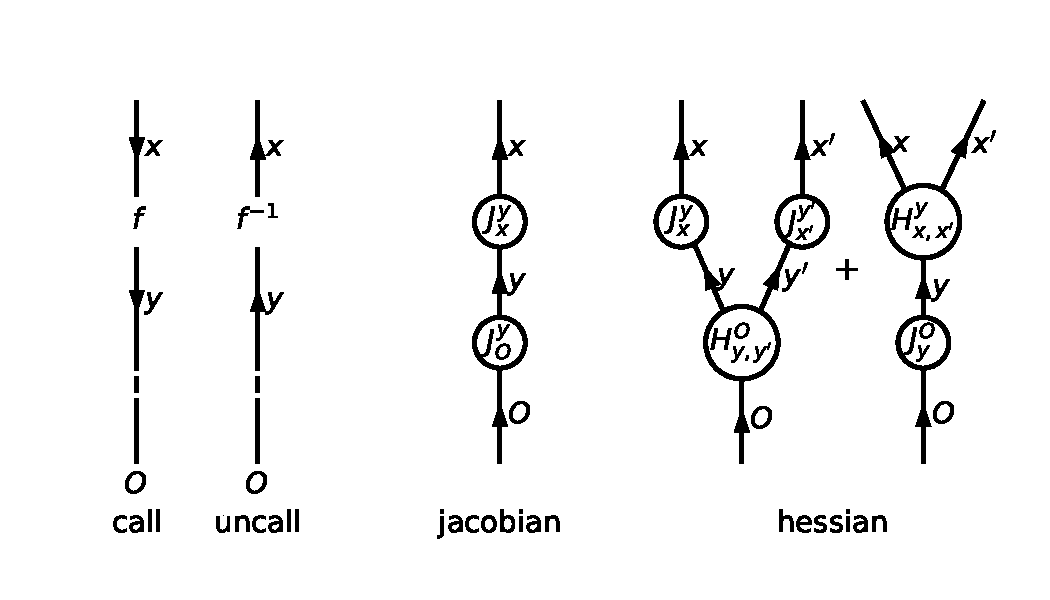
\includegraphics[width=\columnwidth,trim={0 1cm 0 1cm},clip]{images/ad.pdf}}
    \caption{Adjoint rules for Jacobians and Hessians in tensor network language.}\label{fig:ad}
\end{figure}

In reversible programming, we have the following implementation
\begin{enumerate}
    \item The program runs forward and computes outputs,
    \item call constructor \texttt{GVar} that transfer a floating point number type to a \texttt{GVar} type.
    \item Add $1$ to the gradient field of the loss variable,
    \item The program uncomputes outputs and recover all inputs, gradients are the \texttt{grad} fields of input variables.
\end{enumerate}

Here, \texttt{GVar} is a ``reversible type''. \texttt{GVar(x)} wraps a variable into a GVar, which attaches a zero gradient field to a variable just like the dual number in tangent mode automatic differentiation. Its inverse $~GVar$ deallocate the gradient field safely and returns its value field. Here, "safely" means it will check the gradient field to make sure it is in $0$ state.
When a \texttt{instruct} meets a \texttt{GVar}, besides computing its value field $value(\vx) \leftarrow f^{-1}(value(\vy))$, it also updates the gradient field $grad(\vx) = f^{-1}(value(\vx), grad(\vy))$. Since $f^{-1}$ is bijective, $J^\vy_\vx$ can be easily obtained by inspecting its inverse function $f$.
The final output is stored in the gradient field, when then gradient is not used anymore, the faithful reversible programming style to compute gradients would be uncomputing the whole process to obtain gradient, which increases the hyrachy by 1. Whenever the hyrachy increase by 1, the computational overhead doubles comparing with its irreversible counter part.

\subsection{Second order gradient}
The second order gradient can also be back propagated
\begin{align}
    \begin{split}
        &H^f_{y_L,y_L'} = 0\\
        &H^f_{y_{i-1},y_{i-1}'} = J^{y_i}_{y_{i-1}} H^f_{y_i, y_i'} J^{y_i'}_{y_{i-1}'} + J^f_{y_i} H^{y_i}_{y_{i-1}, y_{i-1}'}
    \end{split}
\end{align}

In tensor network language, it can be represented as in \Fig{fig:ad}.
This approach can be easily extended to higher orders, or taylor propagation.
However, this is not the widely adopted approach to compute higher order gradients.
Althought backpropagating higher order gradients directly is exponentially faster than back propagating the computational graph for computing lower order gradients for computing higher order gradients, one has to extending the backward rules for each primitive rather than reusing existing ones.
Here, we emphasis that with instruction level AD, rewritting backward rules for primitives turns out to be not so difficult.

\subsection{Gradient on ancilla problem}
Ancilla can also carry gradients during computation, sometimes these gradients can not be uncomputed even if their parents can be uncomputed regoriously. In these case, we simply ``drop'' the gradient field instead of raising an error. In this subsection, we prove doing this is safe, i.e. does not have effect on rest parts of program.

Ancilla is the fixed point of a function, which means 
\begin{align}
    \begin{split}
    &b, y \leftarrow f(x, a)\; \text{, where } b==a\\
    &\frac{\partial b}{\partial x} = 0
    \end{split}
\end{align}

During the computation, the gradient field does not have any effect to the \texttt{value} field of variables. The key question is will the loss of gradient part in ancilla affect the reversibility of the gradient part of argument variables.
The gradient of argument variable is defined as $\frac{\partial L}{\partial x} = \frac{\partial L}{\partial y}\frac{\partial y}{\partial x} + \frac{\partial L}{\partial b}\frac{\partial b}{\partial x}$, where the second term vanish naturally.

\subsection{Implementation}
The automatic differentiation engine is so short that we present the function defintion as follows

\begin{minipage}{.44\textwidth}
\begin{lstlisting}
@i function (g::Grad)(args...; kwargs...)
    @safe @assert count(x -> x isa Loss, args) == 1
    @anc iloss = 0
    @routine getiloss begin
        for i=1:length(args)
            if (tget(args,i) isa Loss, iloss==i)
                iloss += identity(i)
                (~Loss)(tget(args,i))
            end
        end
    end

    g.f(args...; kwargs...)
    GVar.(args)
    grad(tget(args,iloss)) += identity(1.0)
    (~g.f)(args...; kwargs...)

    ~@routine getiloss
end
\end{lstlisting}
\end{minipage}

The program first checks the input parameters and locate the loss variable.
Then \texttt{~Loss} unwraps the loss variable, the location of loss variable is transferred to the ancilla \texttt{iloss} of integer type.

\texttt{GVar}

\begin{minipage}{.44\textwidth}
\begin{lstlisting}
julia> using NiLang, NiLang.AD

julia> x, y = GVar(0.5), GVar(0.6)
(GVar(0.5, 0.0), GVar(0.6, 0.0))

julia> @instr grad(x) += identity(1.0)

julia> @instr x += identity(y)

julia> y
GVar(0.6, -1.0)

julia> @instr grad(x) -= identity(1.0)

julia> @instr (~GVar)(x)

julia> x
1.1
\end{lstlisting}
\end{minipage}

Broadcasting is supported. To avoid possible confusing, tuple indexing is forbidden delebrately, one can use \texttt{tget(tuple, 2)} to get the second element of a tuple.

\section{Examples}

\section{Computing Fibonacci Numbers}\label{sec:fib}
An example that everyone likes

\begin{minipage}{.44\textwidth}
\begin{lstlisting}
@i function rfib(out, n::T) where T
    @anc n1 = zero(T)
    @anc n2 = zero(T)
    @routine init begin
        n1 += identity(n)
        n1 -= identity(1.0)
        n2 += identity(n)
        n2 -= identity(2.0)
    end
    if (value(n) <= 2, ~)
        out += identity(1.0)
    else
        rfib(out, n1)
        rfib(out, n2)
    end
    ~@routine init
end
\end{lstlisting}
\end{minipage}

To compute the first Fibonacci number that is greater or equal to 100

\begin{minipage}{.44\textwidth}
\begin{lstlisting}
@i function rfib100(n)
    @safe @assert n == 0
    while (fib(n) < 100, n != 0)
        n += identity(1.0)
    end
end
\end{lstlisting}
\end{minipage}

Here, \texttt{fib} and \texttt{rfib} are defined in \App{sec:fib}.
The reversible \texttt{while} statement contains two statements, the precondition and postcondition.
Before entering the while statement, the program check the postcondition to make sure it is false.
After each iteration, postcondition returns true. The inverse function exchanges the precondition and postcondition so that the repeatition of loop body is not changed.

\section{Taylor propagation on a reversible Turing machine}
Taylor propagation is exponentially (as the order) more efficient in obtaining higher order gradients than differentiating lower order gradients recursively.
The later requires traversing the computational graph repeatedly.
In JAX, in order to support Taylor propagation, the propagation rules for part of primitives manually defined.
The exhaused support requires much more effort than the first order gradient propagation.
Instruction level automatic differentiation is more flexible in obtaining higher order gradients like Hessian.


\subsection{exp function}
An $\exp$ function can be computed using Taylor expansion
\begin{equation}
    {\rm out!} += \sum\limits_n \frac{x^n}{n!}
\end{equation}
At a first glance, this is a recursive algorithm that mimics pebble game.
Define the term for accumulation $s_n \equiv \frac{x^n}{n!}$, the recursion relation is written as $s_n = \frac{x s_{n-1}}{n}$.
There is no known constant memory algorihm to pebble game.
Notice that by viewing $*=$ and $/=$ a pair of reversible operations, we can uncompute $s_{n-1} = \frac{n s_n}{x}$ to deallocate memory.
By allowing loss of several digit precision of result, implementing the constant memory reversible $\exp$ function is possible

\begin{minipage}{.44\textwidth}
\begin{lstlisting}
using NiLang, NiLang.AD

@i function iexp(out!, x::T; atol::Float64=1e-14)
        where T
    @anc anc1 = zero(T)
    @anc anc2 = zero(T)
    @anc anc3 = zero(T)
    @anc iplus = 0
    @anc expout = zero(T)

    out! += identity(1.0)
    @routine r1 begin
        anc1 += identity(1.0)
        while (value(anc1) > atol, iplus != 0)
            iplus += identity(1)
            anc2 += anc1 * x
            anc3 += anc2 / iplus
            expout += identity(anc3)
            # speudo inverse
            anc1 -= anc2 / x
            anc2 -= anc3 * iplus
            SWAP(anc1, anc3)
        end
    end

    out! += identity(expout)

    ~@routine r1
end
\end{lstlisting}
\end{minipage}

The definition of SWAP instruction can be found in \App{app:instr}.
The two lines bellow the comment \texttt{\# pseudo inverse} "uncompute" variables \texttt{anc1} and \texttt{anc2} to avalue very close to zero.
Although the final output is not exact due to the rounding error, the reversibility is not harmed.
Rouding error in output is not as toxical as that in ancilla, in the latter case, error accumulates in the whole program.
In the second for loop inside the inverse notation \texttt{\~}, we uncompute all ancilla bits rigorously.
The \texttt{while} statement takes two conditions, the precondition and postconditoin. Precondition \texttt{val(anc1) > atol} indicates when to break the forward pass and post condition \texttt{!isapprox(iplus, 0.0)} indicates when to break the backward pass.

The appendix gives another example of QR decomposition.

To obtain the gradient, one can wrap the loss with \texttt{Loss} type.

\begin{minipage}{.44\textwidth}
\begin{lstlisting}
julia> out!, x = 0.0, 1.6
(0.0, 1.6)

julia> @instr iexp'(Loss(out!), x)

julia> grad(x)
4.9530324244260555

julia> out!, x = 0.0, 1.6
(0.0, 1.6)

julia> @instr iexp''(Loss(out!), x)

julia> collect_hessian()
2×2 Array{Float64,2}:
 0.0  0.0
 0.0  4.95303
\end{lstlisting}
\end{minipage}

\texttt{iexp\textquotesingle} returns an object of type \texttt{Grad{typeof(exp)}}, it is a reversible function.
Due to the non-locality of Hessians, we use a global tape for Hessian propagation. Whenever a new variable is created, the tape allocates a larger ring.
It is global to ease the memory allocations of ancillas, the Hessian in ancilla is important to reach correct result.

\begin{minipage}{.44\textwidth}
\begin{lstlisting}
julia> out!, x = 0.0, 1.6
(0.0, 1.6)

julia> @instr iexp''(Loss(out!), x)

julia> collect_hessian()
2×2 Array{Float64,2}:
 0.0  0.0
 0.0  4.95303
\end{lstlisting}
\end{minipage}

The final result can be obtained by calling a global function \texttt{collect\_hessian}.

\subsection{QR decomposition}

Not only simple functions, linear algebra functions 

\begin{minipage}{.44\textwidth}
\begin{lstlisting}
@i function iqr(Q, R, A::AbstractMatrix{T}) where T
    @anc anc_norm = zero(T)
    @anc anc_dot = zeros(T, size(A,2))
    @anc ri = zeros(T, size(A,1))
    for col = 1:size(A, 1)
        ri .+= identity.(A[:,col])
        for precol = 1:col-1
            idot(anc_dot[precol], Q[:,precol], ri)
            R[precol,col] += identity(anc_dot[precol])
            for row = 1:size(Q,1)
                ri[row] -= anc_dot[precol] * Q[row, precol]
            end
        end
        inorm2(anc_norm, ri)

        R[col, col] += anc_norm^0.5
        for row = 1:size(Q,1)
            Q[row,col] += ri[row] / R[col, col]
        end

        ~(ri .+= identity.(A[:,col]);
        for precol = 1:col-1
            idot(anc_dot[precol], Q[:,precol], ri)
            for row = 1:size(Q,1)
                ri[row] -= anc_dot[precol] * Q[row, precol]
            end
        end;
        inorm2(anc_norm, ri)
        )
    end
end
\end{lstlisting}
\end{minipage}

where \texttt{idot} and \texttt{inorm2} are implemented as

\begin{minipage}{.44\textwidth}
\begin{lstlisting}
@i function idot(out, v1::AbstractVector{T}, v2)
        where T
    @anc anc1 = zero(T)
    for i = 1:length(v1)
        anc1 += identity(v1[i])
        CONJ(anc1)
        out += v1[i]*v2[i]
        CONJ(anc1)
        anc1 -= identity(v1[i])
    end
end

@i function inorm2(out, vec::AbstractVector{T})
        where T
    @anc anc1 = zero(T)
    for i = 1:length(vec)
        anc1 += identity(vec[i])
        CONJ(anc1)
        out += anc1*vec[i]
        CONJ(anc1)
        anc1 -= identity(vec[i])
    end
end
\end{lstlisting}
\end{minipage}

One can easily check the gradient of this naive implementation of QR decomposition is correct

\begin{minipage}{.44\textwidth}
\begin{lstlisting}
using Test
A = randn(4,4)
q = zero(A)
r = zero(A)

@i function test1(out, q, r, A)
    iqr(q, r, A)
    out += identity(q[1,2])
end

@i function test2(out, q, r, A)
    iqr(q, r, A)
    out += identity(r[1,2])
end

@test check_grad(test1, (Loss(0.0), q, r, A);
        atol=0.05, verbose=true)
@test check_grad(test2, (Loss(0.0), q, r, A);
        atol=0.05, verbose=true)
\end{lstlisting}
\end{minipage}

Here, the \texttt{check\_grad} function is a gradient checker function defined in \texttt{NiLangCore.ADCore}.

\subsection{Unitary Matrices}
Recurrent networks with a unitary parametrized network ease the gradient exploding and vanishing problem~\cite{Arjovsky2015,Wisdom2016,Li2016}.
Among different parametrization schemes, the most elegant one is \cite{Li2016}, which parametrized the unitary matrix with two-level unitary operations, any unitary matrix of size $N\times N$ can be parametrized by $k = N(N-1)/2$ two level unitary matrices~\cite{Li2013}. All these two-level unitary matrices can be applied in $O(1)$ time as a two register instruction.
Hence a real unitary matrix can be parametrized compactly by $k$ rotation angles, each represents a rotation operations between datas in two target parameters.


\begin{minipage}{.44\textwidth}
\begin{lstlisting}
@i function umm!(x, θ, Nin::Int, Nout::Int)
    @anc k = 0
    for j=1:Nout
        for i=Nin-1:-1:j
            k += identity(1)
            ROT(x[i], x[i+1], θ[k])
        end
    end

    # uncompute k
    for j=1:Nout
        for i=Nin-1:-1:j
            k -= identity(1)
        end
    end
end
\end{lstlisting}
\end{minipage}

\texttt{ROT(a!, b!, $\theta$)} is the rotation instruction, \texttt{$\theta$} is the rotation angle, which represents rotating data in \texttt{a!} and \texttt{b!} by an angle of $\theta$.

\begin{align}
    R(\theta)  = \begin{bmatrix}
        \cos(\theta) & - \sin(\theta)\\
        \sin(\theta)  & \cos(\theta)
    \end{bmatrix}
\end{align}


Its backward rule of a \texttt{ROT} instruction is
\begin{align}
    \begin{split}
    \overline{\theta}  &= \sum\frac{\partial R(\theta)}{\partial \theta}\odot(\overline{y}x^T)\\
    &= \Tr\left[\frac{\partial R(\theta)}{\partial \theta}^T\overline{y}x^T\right]\\
    &= \Tr\left[R\left(\frac{\pi}{2}-\theta\right)\overline{y}x^T\right]
    \end{split}
\end{align}

We bind the adjoint function of \texttt{ROT} to its reverse \texttt{IROT},
and define a new function that dispatch to \texttt{GVar} variables

\begin{minipage}{.44\textwidth}
\begin{lstlisting}
@i function IROT(a!::GVar, b!::GVar, θ::GVar)
    IROT(value(a!), value(b!), value(θ))
    NEG(value(θ))
    value(θ) -= identity(π/2)
    ROT(grad(a!), grad(b!), value(θ))
    grad(θ) += value(a!) * grad(a!)
    grad(θ) += value(b!) * grad(b!)
    value(θ) += identity(π/2)
    NEG(value(θ))
    ROT(grad(a!), grad(b!), π/2)
end
\end{lstlisting}
\end{minipage}

\section{Training by consistency}
We compute the output as
\begin{equation}
    y = f(x),
\end{equation}
and we have an expected output $\hat{y}$. In traditional machine learning, we define a loss and minimize it. However, this is not how human brain works.~\cite{Hintoncomment}
Since the $\hat{y}$ is different with $y$, the network start to "think", if the output is $\hat{y}$, what should the input (including network parameters) be?
So, we feed $\hat{y}$ back to the output end of network, and inverse the tape, with the runtime information generated by the input image. The network will compute a different value to network parameters, then the network feel "confused", and chose a value between old and new values.

Let's look at the following example
\begin{minipage}{.44\textwidth}
\begin{lstlisting}[basicstyle=\small\ttfamily,columns=fullflexible]
@i function f1(out!, x, y)
    y += identity(x)
    out! -= exp(x)
    out! += exp(y)
end

@i function f2(out!, x, y)
    y += identity(x)
    out! -= exp(x)
    x -= log(-out!)
    out! += exp(y)
end

function train(f)
    loss = Float64[]
    y = 1.6
    for i=1:100
        out!, x = 0.0, 0.3
        @instr f(out!, x, y)
        push!(loss, out!)
        out! = 1.0
        @instr (~f)(out!, x, y)
    end
    loss
end
\end{lstlisting}
\end{minipage}

Loss function \texttt{f1} and \texttt{f2} computes $f(x, y) = e^{(y+x)} - e^x$ and stores the output in a new memory \texttt{out!}, the target is to find a $y$ that make the output $x$ equal to the target value $1$.
After $200$ steps training, $y$ runs into the fixed point and $x$ is equal to $1$ upto machine precision.

\begin{figure}
    \centerline{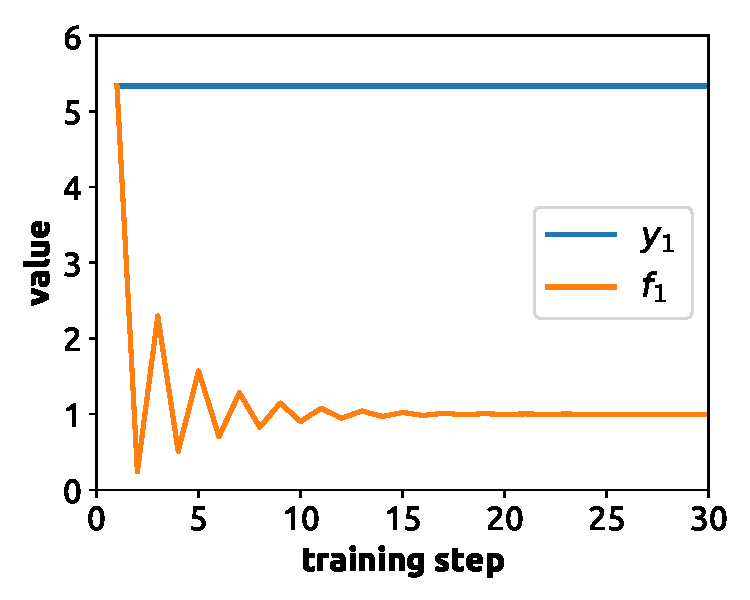
\includegraphics[width=\columnwidth,trim={0 0 0 0},clip]{images/fig1.pdf}}
    \caption{Target function value as a function of self-consistent training step.}\label{fig:invtrain}
\end{figure}

This training is similar the recursive convergence method that widely used in mathematics and physics.
However, in programming language but it has a loophole, it is vulnarable to loss of injectivity.
For example, if the result is accumulated to another variable $z += x$, and take $z$ as the loss, then the loss can not accumulated to the target value correctly since the inverse of above operation is $z -= x$ and $x$ is unchanged in the inverse run.
This is because the redundancy introduced in operation $z = z+e^x$, which keeps both $x$ and $z$, the change of $z$ shifting $z$ directly is apparently a lazier approach to fit $z$ with target value $1$, to figure out the correct causality, corresponding change in output side to $x$ and $y$ are required. This redundancy can be detected by computing the entanglement entropy (or mutual information) between two output datas. We call this type of invertibility inference, which should be avoided in this type of training. Then how shall we calculate $f(x) = e^x$ like functions, which are not partly invertible from the numeric perspective? Here we introduce the notion of "weak invertibility"
\begin{align}
    &@assert y == 0\\
    &\fl(y) += exp(\fl(x))\\
    &\fl(x) -= log(y)
\end{align}
We can keep $x$ to ensure numerical invertibility, meanwhile erase most informations inside it. Since $x$ is effectively $0$, thus no redundancy (or entanglement entropy) in output, in this way, the above training is still valid.

\subsection{Compactness of data}
Measure of compactness by entanglement entropy.
In invertible programming, we define the entanglement between output space garbage space as the compactness of information.

If the output information is compact, then we have
$(x, x_a)\rightarrow (y, y_a)$

mutual information is
\begin{align}
    I(x, y) = S(x, y) - S(x) - S(y)\\
    S(x, x_a) = S(y, y_a)\\
    I(x, x_a) = 0\\
    I(y, y_a) = S(y, y_a) - S(y_a)
\end{align}

\subsection{Traditional Invertible Computing Devices}
It is possible to design and fabricate a fully reversible processor using resources which are comparable to a conventional microprocessor. Existing CAD tools and silicon technology are sufficient for reversible computer design.

Like quantum computer, it should be able to reset to qubits $0$. The reset operation, sometimes can be expensive. In a quantum device, this reset operation can be done by dissipation and dicoherence (i.e. interact with environment and get thermalized). Alternatively, a immediate feedback loop can be introduced to a quantum device, where a classical computer is regarded as the dissipation source.

\section{Discussion and outlook}

This could be used to reduce the momory cost in normalizing flow, time reversible integrator, recurrent neural network and residual neural network.
\subsection{Time Space Tradeoff}
So far, we have introduced the eDSL. There are many other designs of reversible language and instruction set.
The reversible Turing machine may have either a space overhead propotional to computing time $T$ or a computational overhead that sometimes can be even exponential given limited space.
In the simplest g-segment trade off scheme~\cite{Bennett1989,Levine1990}, it takes $Time(T) = T^{\log _g(4g-2)}$ and $Space(T) = (g-1)S\log_g T$.
This section, we try to convince the reader that the overhead of reversible computing is not as terrible as people thought.

First, one should notice that even in the worst case, the overhead of a reversible program is not more than a traditional machine learning package. In pytorch, a tensor memorize every input of a primitive. The program is apparently reversible since it does not discard any information.
For deep neural networks, people used checkpointing trick to trade time with space~\cite{Chen2016}, which is also a widely used trick in reversible programming~\cite{Perumalla2013}. Reversible programming AD is sometimes more memory efficient. Comparing with logging computational graph, reversible programming has the advantage of supporting inplace functions, which is difficult is both tranditional and source to source AD framework. The example of parametrizing unitary matrice costs zero memory allocation.

Second, some computational overhead of running recursive algorithms with limited space resources can be mitigated by "pseudo uncomputing" without sacrifising reversibility like in the \texttt{iexp} example.

Third, making reversible programming an eDSL rather than a independant language allows flexible choices between reversibility and computational overhead. For example, in order to deallocate the gradient memory in a reversible language one has to uncompute the whole process of obtaining this gradient.
In this eDSL, we can just deallocate the memory irreversibly, i.e. trade energy with time. This underlines the fact that a reversible program is more suited in a program with small granularity. We can quantify it by introducing
\begin{definition}[program granularity]
    The logarithm of the ratio between the execution time of a reversible program and its irreversible counter part.
    \begin{equation}
        \log_2 \frac{Time(T)}{T}
    \end{equation}
\end{definition}

In the lowest granuality, instruction design, we need ancilla bits. Defining primitive functions like \texttt{iexp} requires uncomputing ancillas. Deallocating the gradient further increase the granularity by $\sim 1$. After the training, the inverse training of whole programs should be done to deallocate all the memory used for training. As a result, the program complexity increase exponentially as the granuality increase.
The granularity can be decreased by flattening the functions, since the uncomputing of ancillas can be executed at any level of granularity.

One should notice the memory advantage of reversible programming to machine learning does comes from reversibility itself, but from a better data tracking strategy inspired from invertible programming.
Normally, a reversible program is not as memory efficient as its irreversible couterpart due to the additional requirement of no information loss. A naive approach that keeping track of all informations will cost an additional space $O(T)$, where $T$ stands for the excution time in a irreversible TM, the longer the program runs, the larger the memory usage is. This is exactly the approach to keeping reversibility in most machine learning packages in the market.
The point it, an reversible Turing Machine is able to trade space with time.
In some cases, it may cause polynomial overhead than its irreversible counterpart.

\subsection{Instructions and Hardwares}
%Todays CPU are starving, that is, the memory access is the performance bottleneck in many applications rather than the arithmetic operations.
%There is a natural granularity for operations with memory access or not.
So far, our eDSL is not really compiled to instructions, instead it runs on a irreversible host Julia.
In the future, it can be compiled to low level instructions and is executable on a reversible devices.
For example, the control flow defined in this NiLang can be compiled to reversible instructions like conditioned \texttt{goto} statement.
It is designed in such a way that the target instruction is a \texttt{comefrom} statement which specifies the postcondition. ~\cite{Vieri1999}

Arithmetic instructions should be redesigned to support better reversible programs.
The major obstacle to exact reversibility programming is current floating point adders used in our computing devices are not exactly reversible.
There are proposals of reversible floating point adders~\cite{Nachtigal2011,Nguyen2013} that introduces garbage bits to ensure reversibility.
In other words, to represent a 64 bit floating point number requires more than 64 bits in storage. Reversible multiplier is also possible in similar approach.~\cite{Nachtigal2010} With these infrastructure, a reversibile program can be executed without suffereing from the irreversibility from rounding error.
In machine learning field, people using information buffer in multiplication operations~\cite{Maclaurin2015} in an approach to enforce invertibility in a memory efficient way.

Reversible programming is not nessesarily related to reversible hardware, reversible programs are a subset of irreversible programs hence can be simulated efficiently with CMOS technologies. However, using reversible hardwares can break the energy efficiency barrier introduce by Landauer principle.
Reversible hardware is not nessesarily related to reversible gates such as Toffoli gate and Fredkin gate.
Devices with the ability of recovering signal energy is able able to save energy, or what we call generalized reversible computing.~\cite{Frank2005,Frank2017b}
In the following, we comment briefly on a special type of reversible device Quantum computer.

\subsection{Quantum Computers}
One of the fundamental difficulty of building a quantum computer is, unlike a classical state, an unknown quantum state can not be copied.
A quantum state in a environment will decoherence and can not be recovered, this underlines the simulation nature of a quantum device.
In the era of noisy intermediate sized quantum devices, more and more people are switching to classical-quantum hybrid devices, where a quantum device plays the role of a programmable simulator.
Reversible computing does not enjoy the supremacy from quantum entanglement, nor the quantum limitations of non-cloning.
Only the limitation of reversibility is retained, reversibility comes from the fact that micro scopic processes are all unitary.
Irreversibility can only come from the interaction with classical devices, like environment induces decaying, qubit state resetting, measurements and classical feedbacks to quantum devices. These are rare resources in microscopic world as well as one of the most difficult part to implement in a practical device.

Quantum gates can possiblely simplify reversible instructions design, e.g. the quantum fourier transformation based adder.
A classical in, classical out algorithm can find a quantum shortcut.
With respect to this fact, it is reasonable to believe there would be a classical-quantum intermediate statge of computing,
the reversible computing that bridge the gap between classical bits and fully entangled qubits.
Although weaker than both, but with a killer application of instruction level automatic differentiation.
By introducing quantum entanglement little by little, we will have faster instructions like addition and multiplication by utilizing quantum fourier transformation, faster algorithms and finally have an application that has genuine quantum advantage.

Reversible Turing machine and rotation gates $Ry(\theta)$ and $Rz(\theta)$ is equivalent to a quantum universal computer.
In NiLang, we implement a path-integral based universal quantum simulator as shown in \App{app:quantum}. It is different from the classical-quantum hybrid mode compiler that using classical control flows, its control flow is reversible, and will be runable on a quantum computer in the future.
The compiling theory developed for reversible programming will have profounding effect to quantum computers.

So far NiLang is not full ready for productivility. It can be improved from multiple perspectives, compiling support to merge the uncomputing can decrease granularity and hence reduce overhead. Additional instructions like stack operations and logical operations are under consideration. It is also interesting to see how it can be combined with a high performance quantum simulator like \texttt{Yao}. It is able to provide control flow to \texttt{Yao}'s QBIR. By porting a quantum simulator. it is interesting to see how quantum simulator can improve the instruction design. Notice a quantum adder is more efficient than a classical adder.

\section{acknowledgments}
Jin-Guo Liu thank Lei Wang for motivating the project with possible applications reversible integrator, normalizing flow and neural ODE.
Xiu-Zhe Luo for discussion on the implementation details of source to source automatic differetiation,
Shuo-Hui Li for helpful discussion on differential geometry.
Damian Steiger for telling me the \texttt{comefrom} joke.
The authors are supported by the National Natural Science Foundation of China under the Grant No.~11774398, the Strategic Priority Research Program of Chinese Academy of Sciences Grant No.~XDB28000000 and the research funding from Huawei Technologies under the Grant No.~YBN2018095185.

\bibliographystyle{apsrev4-1}
\bibliography{invc}

\pagebreak
\appendix

\section{NiLang Grammar}\label{app:grammar}

Terminologies
\begin{itemize}
    \item $ident$, symbols
    \item $num$, numbers
    \item $\epsilon$, empty statement
    \item $JuliaExpr$, native julia expression
    \item $[$ $]$,  zero or one repetitions.
\end{itemize}

\begin{minipage}{0.3\textwidth}
    \small
\begin{bnf*}
    \bnfprod{Stmts}{\bnfsp \bnfes}\\
    \bnfmore{\bnfor \bnfpn{Stmt}}\\
    \bnfmore{\bnfor \bnfpn{Stmts} \bnfsp \bnfpn{Stmt}}\\
    \bnfprod{Stmt}{\bnfpn{BlockStmt}}\\
    \bnfmore{\bnfor \bnfpn{IfStmt}}\\
    \bnfmore{\bnfor \bnfpn{WhileStmt}}\\
    \bnfmore{\bnfor \bnfpn{ForStmt}}\\
    \bnfmore{\bnfor \bnfpn{InstrStmt}}\\
    \bnfmore{\bnfor \bnfpn{RevStmt}}\\
    \bnfmore{\bnfor \bnfpn{@anc} \bnfsp \bnfpn{Stmt}}\\
    \bnfmore{\bnfor \bnfpn{@routine} \bnfsp \bnfpn{Stmt}}\\
    \bnfmore{\bnfor \bnfpn{@safe} \bnfsp \bnftd{$JuliaExpr$}}\\
    \bnfmore{\bnfor \bnfpn{CallStmt}}\\
    \bnfprod{BlockStmt}{\bnftd{begin} \bnfsp \bnfpn{Stmts} \bnfsp \bnftd{end}}\\
    \bnfprod{RevCond}{\bnftd{(} \bnfsp \bnftd{$JuliaExpr$} \bnfsp \bnftd{,} \bnfsp \bnftd{$JuliaExpr$} \bnfsp \bnftd{)}}\\
    \bnfprod{IfStmt}{\bnftd{if} \bnfsp \bnfpn{RevCond} \bnfsp \bnfpn{Stmts} \bnfsp \bnfts{[} \bnftd{else} \bnfsp \bnfpn{Stmts}\bnfts{]} \bnfsp \bnftd{end}}\\
    \bnfprod{WhileStmt}{\bnftd{while} \bnfsp \bnfpn{RevCond} \bnfsp \bnfpn{Stmts} \bnfsp \bnftd{end}}\\
    \bnfprod{Range}{\bnftd{$JuliaExpr$} \bnfsp \bnftd{:} \bnfsp \bnftd{$JuliaExpr$} \bnfsp \bnfts{[} \bnftd{:} \bnfsp \bnftd{$JuliaExpr$}\bnfts{]}}\\
    \bnfprod{ForStmt}{\bnftd{for} \bnfsp \bnftd{ident} \bnfsp \bnftd{=} \bnfsp \bnfpn{Range} \bnfsp \bnfpn{Stmts} \bnfsp \bnftd{end}}\\
    \bnfprod{CallStmt}{\bnftd{$JuliaExpr$} \bnfsp \bnftd{(} \bnfsp \bnfts{[} \bnfpn{DataViews}\bnfts{]} \bnfsp \bnftd{)}}\\
    \bnfprod{Constant}{\bnftd{num} \bnfor \bnftd{$\pi$}}\\
    \bnfprod{InstrBinOp}{\bnftd{+=} \bnfor \bnftd{-=} \bnfor \bnftd{$\veebar$=}}\\
    \bnfprod{InstrTrailer}{\bnfts{[} \bnftd{.}\bnfts{]} \bnfsp \bnftd{(} \bnfsp \bnfts{[} \bnfpn{DataViews}\bnfts{]} \bnfsp \bnftd{)}}\\
    \bnfprod{InstrStmt}{\bnfpn{DataView} \bnfsp \bnfpn{InstrBinOp} \bnfsp \bnftd{ident} \bnfsp \bnfts{[} \bnfpn{InstrTrailer}\bnfts{]}}\\
    \bnfprod{RevStmt}{\bnftd{$\sim$} \bnfsp \bnfpn{Stmt}}\\
    \bnfprod{@routine}{\bnftd{@routine} \bnfsp \bnftd{ident} \bnfsp \bnfpn{Stmt}}\\
    \bnfprod{AncArg}{\bnftd{ident} \bnfsp \bnftd{=} \bnfsp \bnftd{$JuliaExpr$}}\\
    \bnfprod{@anc}{\bnftd{@anc} \bnfsp \bnfpn{AncArg}}\\
    \bnfmore{\bnfor \bnftd{@deanc} \bnfsp \bnfpn{AncArg}}\\
    \bnfprod{@safe}{\bnftd{@safe} \bnfsp \bnftd{$JuliaExpr$}}\\
    \bnfprod{DataViews}{\bnfsp \bnfes}\\
    \bnfmore{\bnfor \bnfpn{DataView}}\\
    \bnfmore{\bnfor \bnfpn{DataViews} \bnfsp \bnftd{,} \bnfsp \bnfpn{DataView}}\\
    \bnfprod{DataView}{\bnfpn{DataView} \bnfsp \bnftd{[} \bnfsp \bnftd{$JuliaExpr$} \bnfsp \bnftd{]}}\\
    \bnfmore{\bnfor \bnfpn{DataView} \bnfsp \bnftd{.} \bnfsp \bnftd{ident}}\\
    \bnfmore{\bnfor \bnftd{$JuliaExpr$} \bnfsp \bnftd{(} \bnfsp \bnfpn{DataView} \bnfsp \bnftd{)}}\\
    \bnfmore{\bnfor \bnfpn{Constant}}\\
    \bnfmore{\bnfor \bnftd{ident}}\\
\end{bnf*}

\end{minipage}

Dataview is a special bijective mapping of an object or a field (or item) of an object.
The dataview can feedback to parent data with the 
\texttt{chfield} method, so that the modified object can generate desired dataview.

\section{Instruction Table}\label{app:instr}
Even though \texttt{$\oplus(identity)$}, \texttt{$\oplus(*)$}, \texttt{$\oplus(/)$} and their reverse together with control flows are sufficient to write an arbituary differentiable program.
For convinience we provide more,
\begin{table}[h!]\centering
\begin{minipage}{\columnwidth}
\ra{1.3}
    \scalebox{1.0}{
        \begin{tabularx}{\textwidth}{X X}\toprule
            ${\rm SWAP}(a, b) \rightarrow b, a$\\
            ${\rm ROT}(a, b, \theta) \rightarrow a \cos\theta - b\sin\theta, b \cos\theta + a\sin\theta, \theta$\\
            ${\rm IROT}(a, b, \theta) \rightarrow a \cos\theta + b\sin\theta, b \cos\theta - a\sin\theta, \theta$\\
            $y \pluseq a^\wedge b \rightarrow y+a^b, a, b$\\
            $y \pluseq \exp(x) \rightarrow y+e^x, x$\\
            $y \pluseq \log(x) \rightarrow y+\log x, x$\\
            $y \pluseq \sin(x) \rightarrow y+\sin x, x$\\
            $y \pluseq \cos(x) \rightarrow y+\cos x, x$\\
            $y \pluseq {\rm abs}(x) \rightarrow y+ |x|, x$\\
            ${\rm NEG}(y) \rightarrow -y$\\
            ${\rm CONJ}(y) \rightarrow y'$\\
            \bottomrule
        \end{tabularx}
    }
    \caption{A collection of reversible instructions.}\label{tbl:revstatements}
\end{minipage}
\end{table}


\section{Julia based eDSL implementation details}

Macro `invfunc` defines a invertible function, ancillas are binded to a function, since ancillas are umcomputed to $0$ at the end of call, so that it can be used repeatedly in a function, it is like a class variable in a class, with no side effects. When the $JuliaExpr$ is a function all, it must be pure.

Some variables can be uncomputed to $0$, but we choose not to for performance reason. For example
\texttt{infer!(argmax, i, x)} which computes the location of maximum value in $x$ and store the output to $i$, if we uncompute it, it doubles additional computational time. Here, we trade off the memory with computation time. As a result, we must feed \texttt{imax} to the function, so that this variable can be manipulated in outer scopes.

%\end{multicols}
\end{document}
